\section{Simulations}\label{V}

In this part, we will illustrate the computational properties of the presented methods.
In particular, we are interested in computing an estimation of the quadratic error of the estimator given by the posterior mean for different values of $\eta$, the iteration parameter, and compare it to the error obtained with oracle estimators.
We also compare the adaptive estimators to their oracle counterpart, obtained by truncating them at the index minimizing the mean square error.
\textcolor{red}{THE PROPER NAME IS NOT ORACLE HERE AS IT DEPENDS ON $\omega$ HOW SHOULD I CALL IT ? SHOULD I FORMULATE IT FOR EACH $\omega$ ?}
In other words, given an estimator $\widehat{\theta}$ of $\theta^{\circ}$, we define $\widehat{\theta}^{\circ}$ for each realization $y$ of $Y$ as follows :
\begin{align*}
m_{y}^{\circ} &:= \min \left\{\argmin\limits_{m \in \left\llbracket 1, G_{\epsilon} \right\rrbracket} \left\{\sum\limits_{j = 1}^{\infty} \left( \left(\widehat{\theta}_{j} \mathds{1}_{\left\{j \leq m\right\}} + \theta^{\times} \mathds{1}_{\left\{j > m\right\}}\right) - \theta^{\circ}\right)^{2}\right\}\right\},\\
\widehat{\theta}^{\circ} &:= \widehat{\theta}_{j} \mathds{1}_{\left\{j \leq m_{y}^{\circ}\right\}} + \theta^{\times} \mathds{1}_{\left\{j > m_{y}^{\circ}\right\}}.
\end{align*}

In particular we call "oracle projection estimator" the sequence obtained this way when $\left(\widehat{\theta}_{j}\right)_{j \in \mathbb{N}} = \left(\frac{Y_{j}}{\lambda_{j}} \mathds{1}_{\left\{j \in \left\llbracket 1, G_{\epsilon} \right\rrbracket \right\}} + \theta^{\times}_{j} \mathds{1}_{\left\{j \in \left\llbracket G_{\epsilon}, \infty \right\rrbracket \right\}}\right)_{j \in \mathbb{N}};$ and "oracle Bayes estimator" the sequence obtained this way when $\left(\widehat{\theta}_{j}\right)_{j \in \mathbb{N}} = \mathbb{E}_{\boldsymbol{\theta}, M \vert Y^{1}}\left[\boldsymbol{\theta}\right].$

\medskip

The simulation protocole is the following :

\begin{algorithm}[H]
\KwData{$\epsilon_{1}$ maximal value for $\epsilon$, $\epsilon_{2}$ minimal value for $\epsilon$, $\theta^{\circ}$, $\lambda$, $\theta^{\times}$, $s$, $\eta$, $N_{exp}$ number of Monte-Carlo experiences, $N$ number of intermediate values for $\epsilon$ between $\epsilon_{1}$ and $\epsilon_{2}$.}
\KwResult{$\widehat{\mathcal{R}_{\mathbb{L}^{2}}}\left(\widehat{\theta}, \theta^{\circ}\right)$ estimation of the mean square error of $\widehat{\theta}$ for each value of $\epsilon$ with the specified true parameters $\theta^{\circ}$, $\widehat{\mathbb{P}}_{M\vert Y}$ estimation of the average distribution of $M \vert Y$ for each value of $\epsilon$ for the specified true parameter $\theta^{\circ}$.}

Generate $\left(\boldsymbol{e}_{j}\right)_{j \in \llbracket 1, N_{exp}\rrbracket}$ vectors of length $\left\lfloor\frac{1}{\epsilon_{2}}\right\rfloor$ whose elements are realizations of $\mathcal{N}(0, 1)$

Initiate $\widehat{\mathcal{R}_{\mathbb{L}^{2}}}\left(\widehat{\theta}, \theta^{\circ}\right)$ as a vector of zeros of length $N$

Initiate $\widehat{\mathbb{P}}_{M\vert Y}$ as a vector of zeros of length $N$

\For{$n \in 1 : N$}{
	$\epsilon := \epsilon_{2} - n \cdot \frac{\epsilon_{2} - \epsilon_{1}}{N}$
	
	\For{$k \in 1 : N_{exp}$}{
		\begin{align*}
		y &:= \left(\lambda_{j} \cdot \theta^{\circ}_{j}\right)_{j \in \left\llbracket1, \left\lfloor\frac{1}{\epsilon}\right\rfloor \right\rrbracket} + \sqrt{\epsilon} \cdot \left(\boldsymbol{e}_{k, j}\right)_{j \in \left\llbracket 1, \left\lfloor\frac{1}{\epsilon}\right\rfloor \right\rrbracket}\\
		\widehat{\mathbb{P}}_{M\vert Y} &= \widehat{\mathbb{P}}_{M\vert Y} + \frac{\left(\mathbb{P}_{M\vert Y = y}(M = m)\right)_{m \in \llbracket1, G_{\epsilon}\rrbracket}}{N_{exp}}\\
		\widehat{\theta} &:= \mathbb{E}\left[\boldsymbol{\theta}^{M}\vert Y=y\right]\\
		\widehat{\mathcal{R}_{\mathbb{L}^{2}}}\left(\widehat{\theta}, \theta^{\circ}\right)_{n} &= \widehat{\mathcal{R}_{\mathbb{L}^{2}}}\left(\widehat{\theta}, \theta^{\circ}\right)_{n} + \frac{\left(\sum\limits_{j = 1}^{\infty} \left(\theta^{\circ}_{j} - \widehat{\theta}_{j}\right)^{2}\right)}{N_{exp}}
		\end{align*}
	}
}
\end{algorithm}

Results of those simulations are represented in \textsc{\autoref{EQM}}.
We see that in every situation, the Bayesian method outperforms the model selection.
This might be due to the choice of the penalization constant fixed to $3$ here.

\medskip

In cases where $\theta^{\circ}$ is polynomial, the Bayesian method does not perform badly compared to the oracle estimates, even in the case where $\lambda$ is exponentially decreasing, which let suppose that the goal to weaken the hypothesis on $\lambda$ is reachable.

However, when $\theta^{\circ}$ decreases exponentially, the adaptive estimates are easily outperformed by the oracle ones.
The adaptive methods estimate way too many parameters in this case.
This phenomenon is followed by an important numerical instability at values of $\epsilon$ where $G_{\epsilon}$ increases (note that the bayesian method seems to be more resistant to it).

\begin{figure}
\centering
\begin{subfigure}{.5\textwidth}
  \centering
  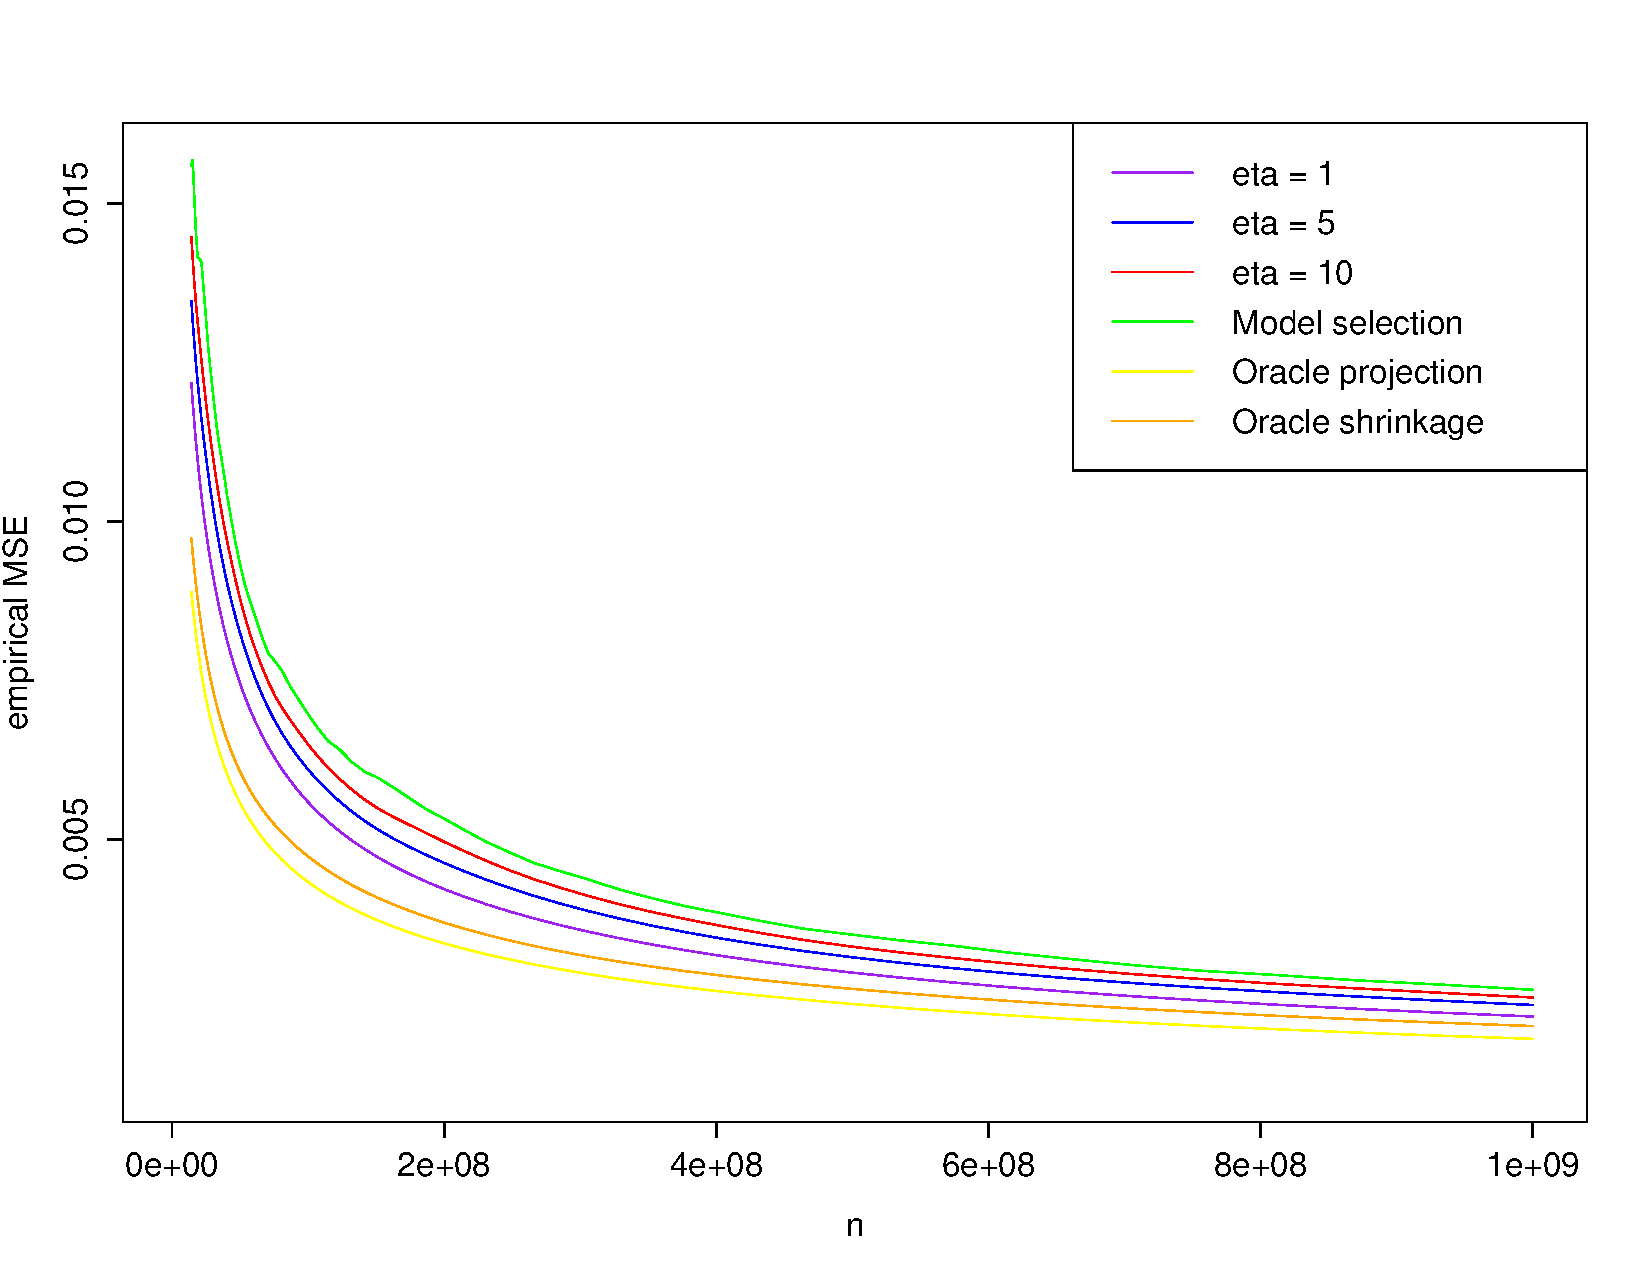
\includegraphics[width=1.\linewidth]{EQM1.pdf}
  \caption{$\theta^{\circ}$ polynomial and $\lambda$ polynomial}
  \label{fig3:sub1}
\end{subfigure}%
\begin{subfigure}{.5\textwidth}
  \centering
  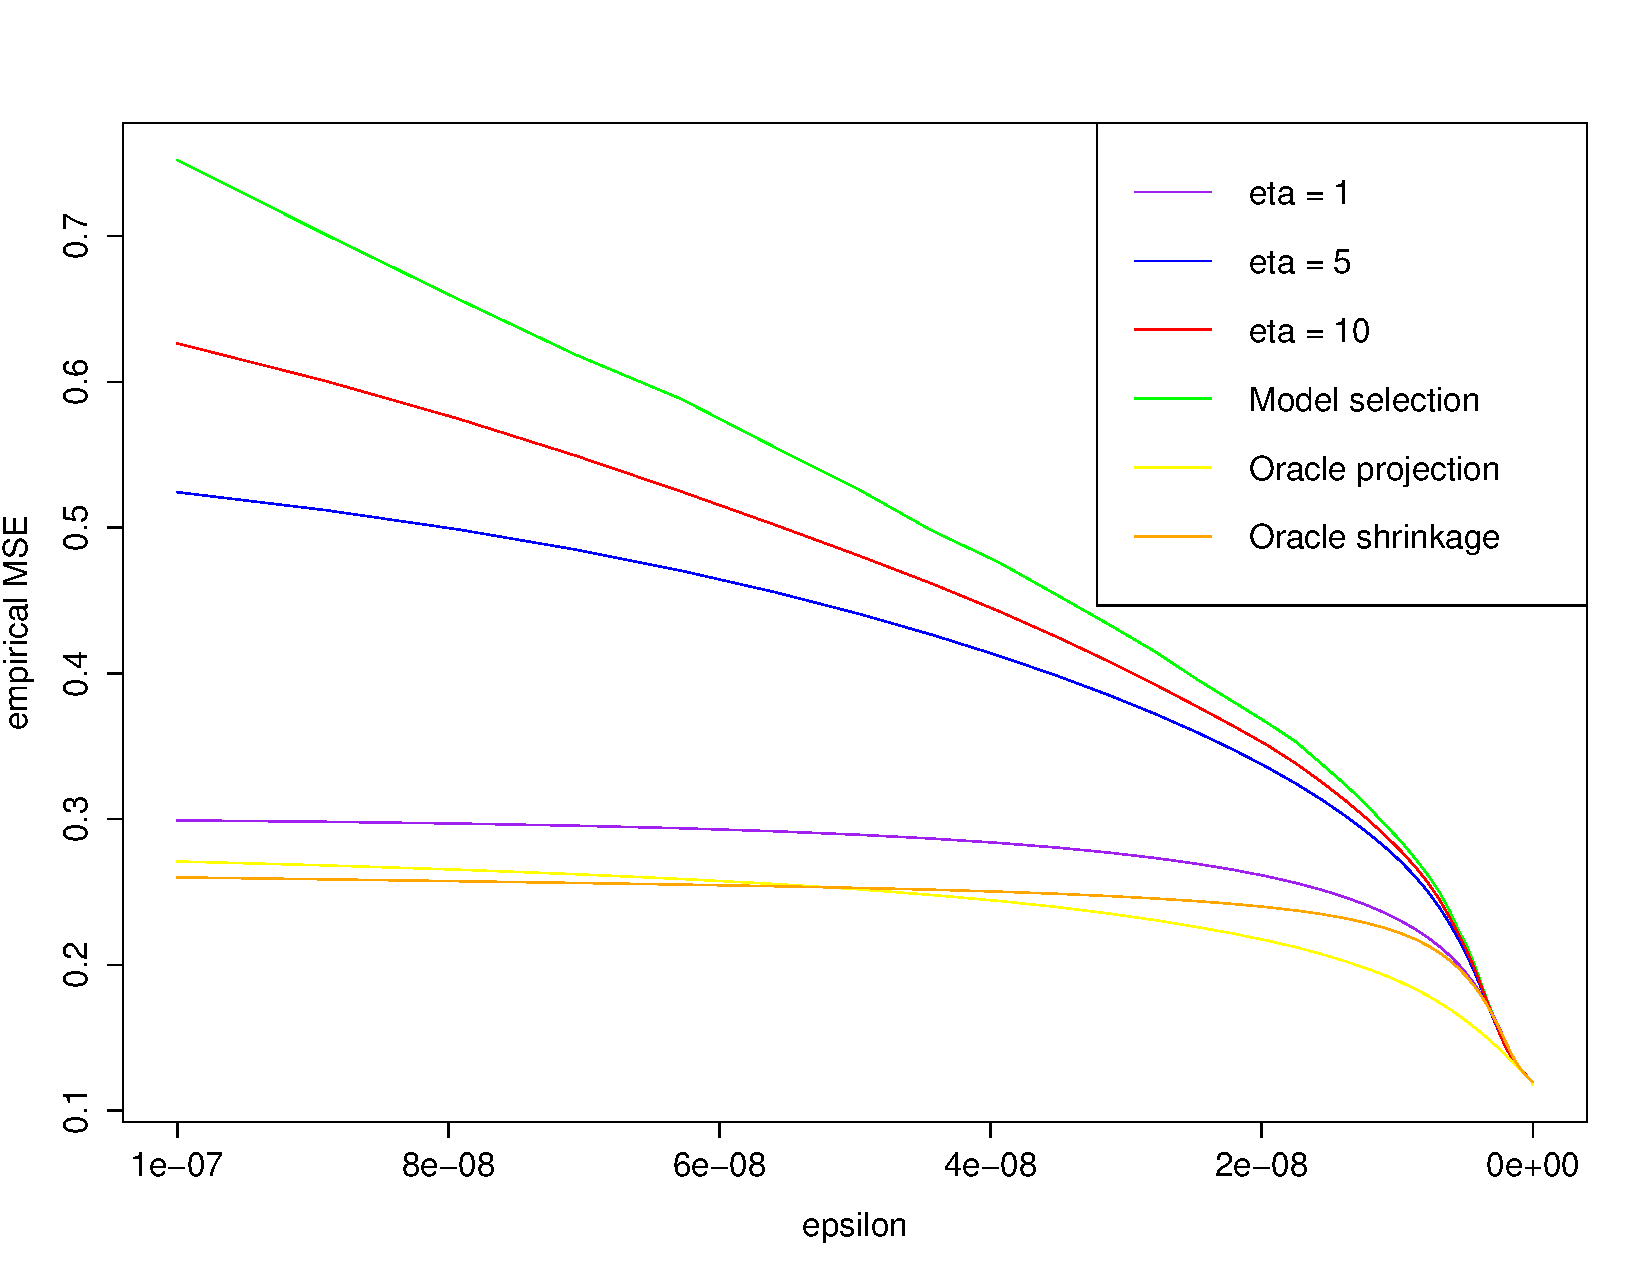
\includegraphics[width=1.\linewidth]{EQM2.pdf}
  \caption{$\theta^{\circ}$ polynomial and $\lambda$ exponential}
  \label{fig3:sub2}
\end{subfigure}
\begin{subfigure}{.5\textwidth}
  \centering
  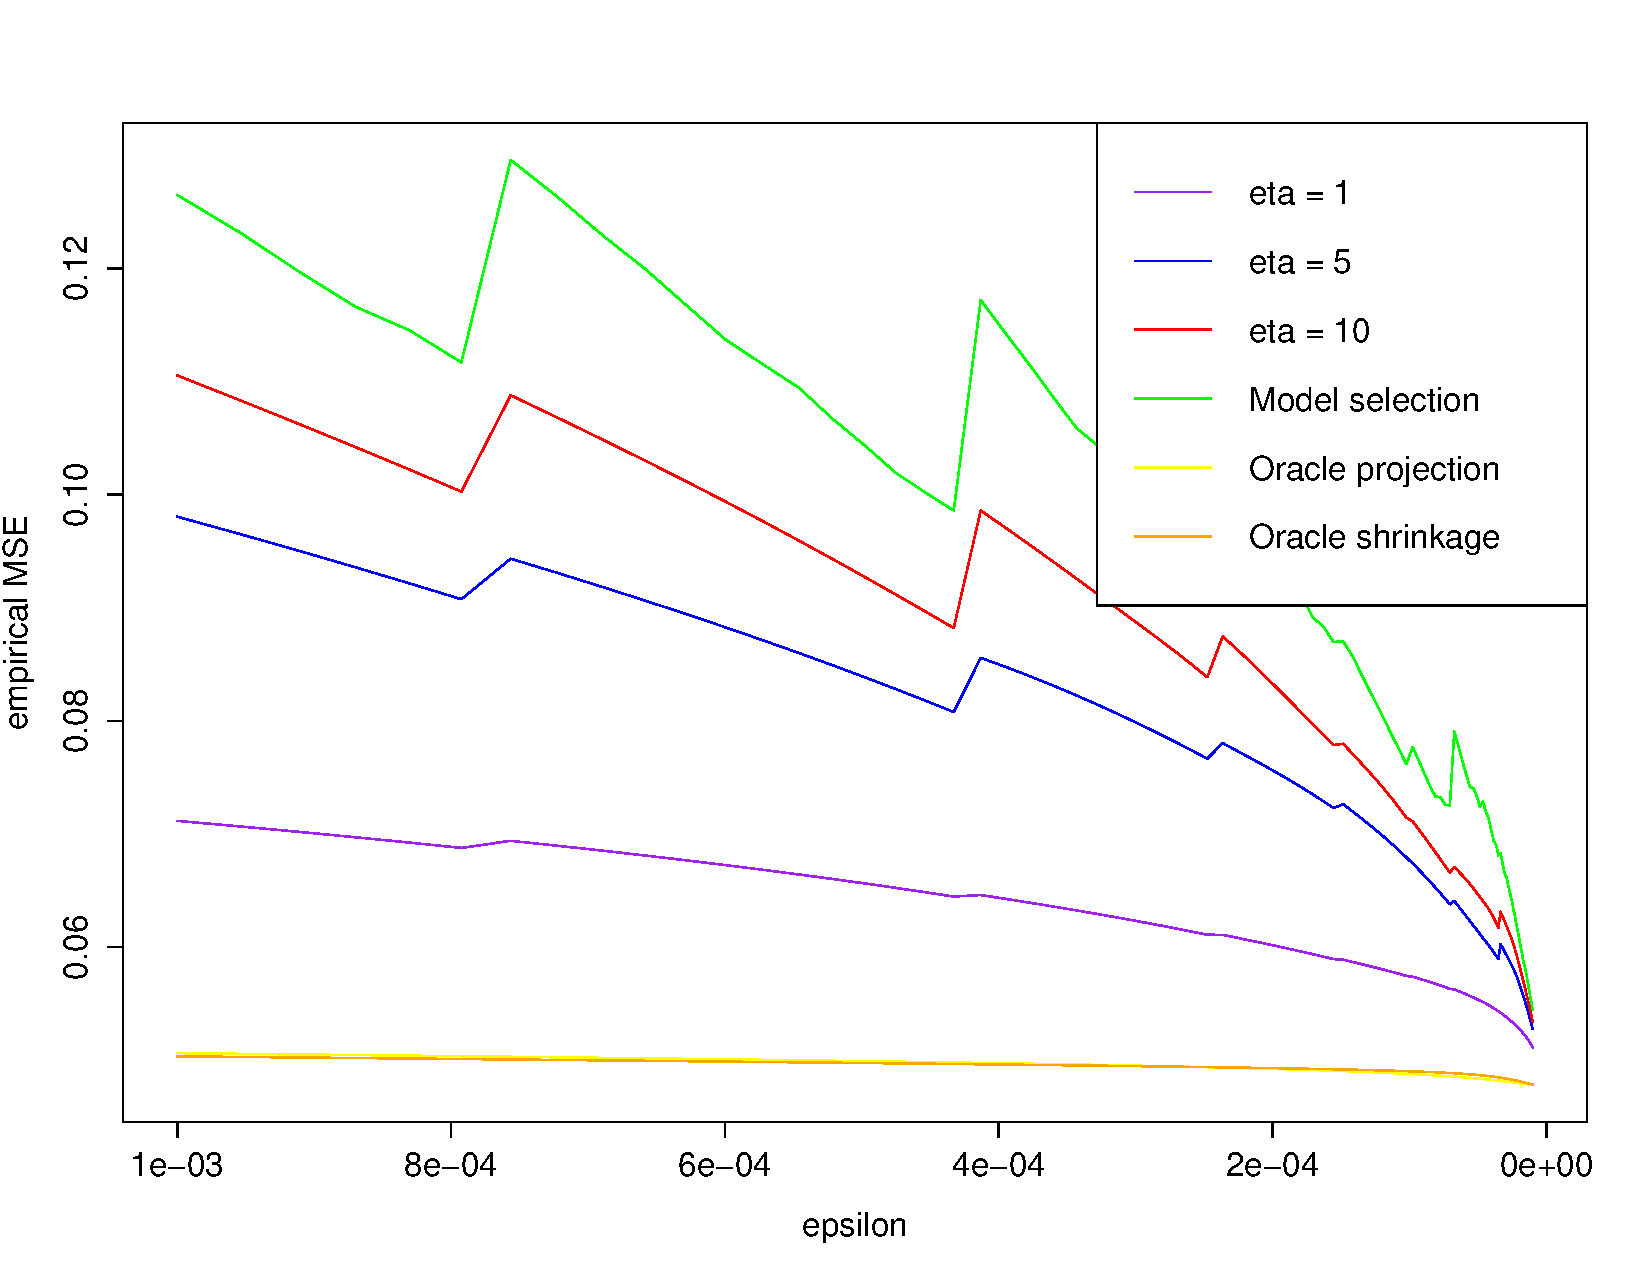
\includegraphics[width=1.\linewidth]{EQM3}
  \caption{$\theta^{\circ}$ exponential and $\lambda$ polynomial}
  \label{fig3:sub3}
\end{subfigure}%
\begin{subfigure}{.5\textwidth}
  \centering
  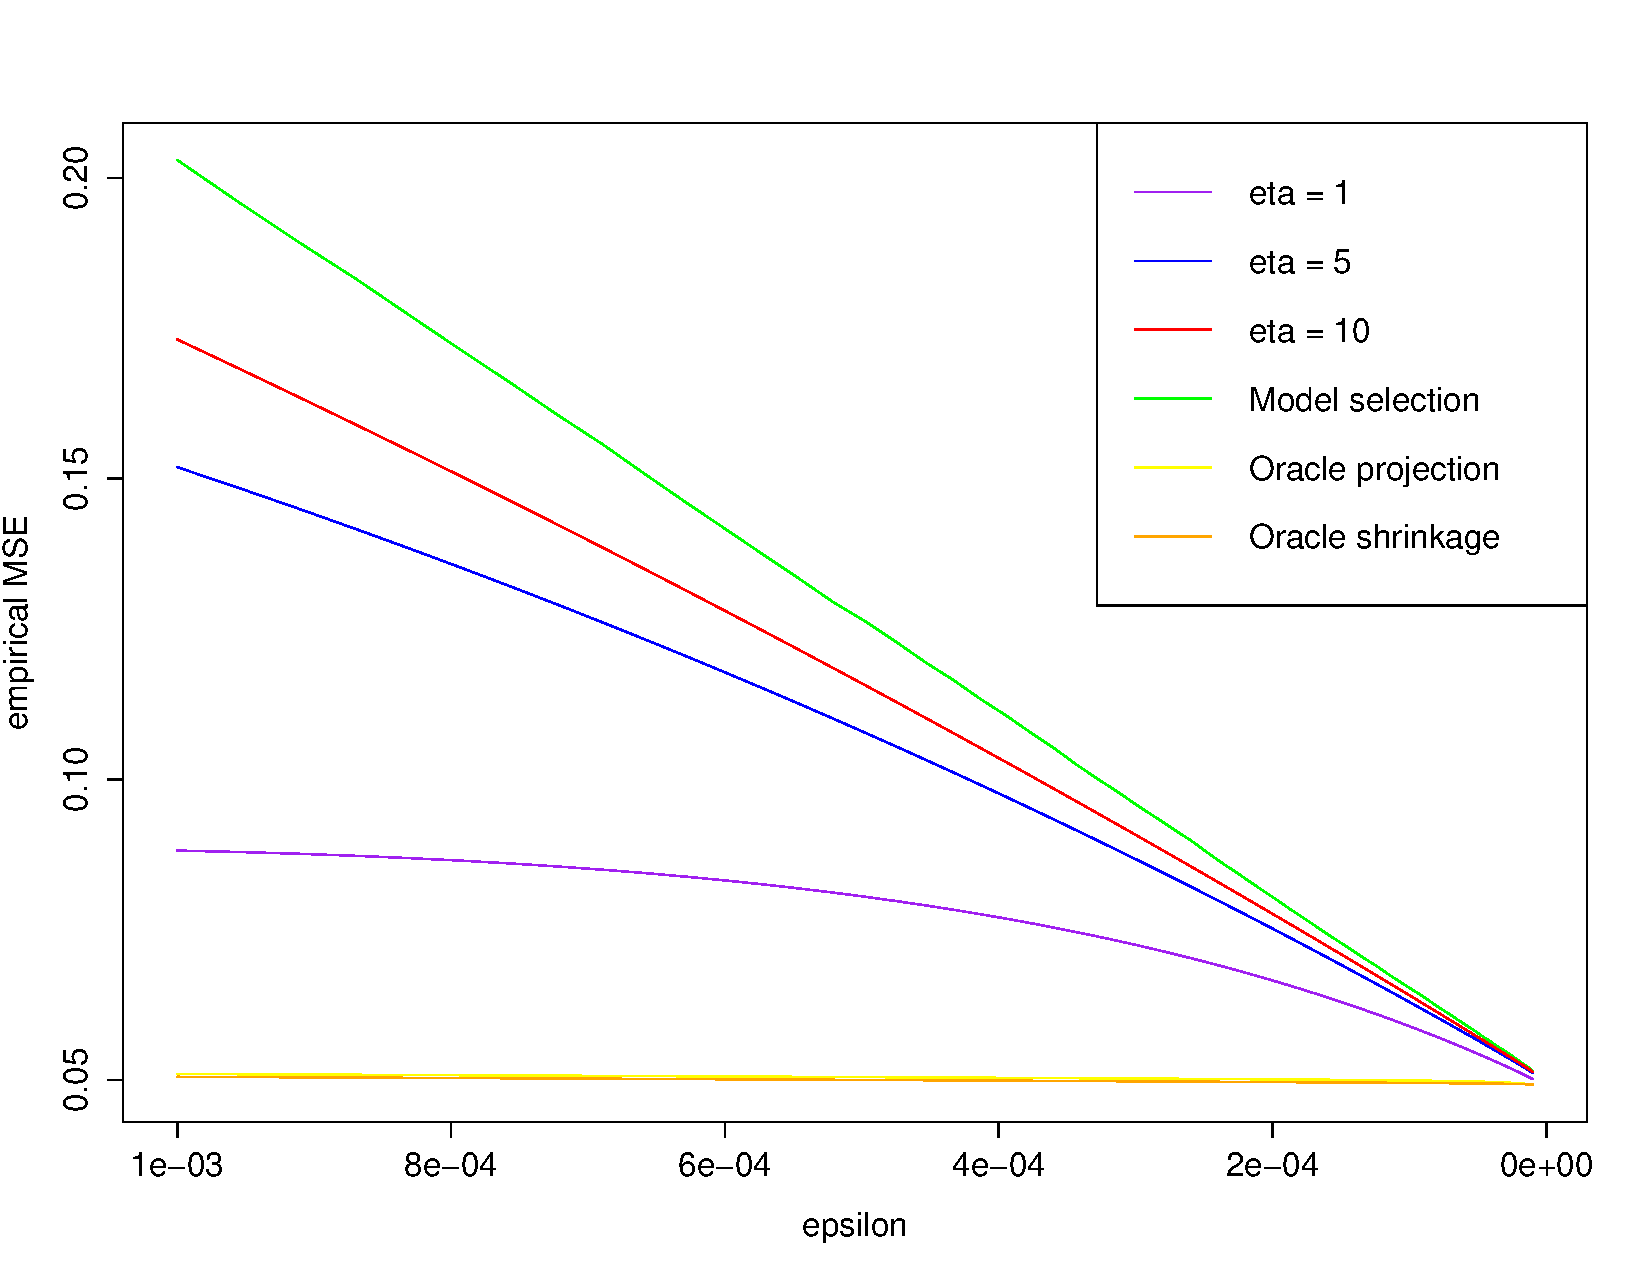
\includegraphics[width=1.\linewidth]{EQM4}
  \caption{$\theta^{\circ}$ exponential and $\lambda$ exponential}
  \label{fig3:sub4}
\end{subfigure}
\caption{Estimated median of the quadratic error of the estimator given by the posterior mean for different classes of $\theta^{\circ}$ and $\lambda$ with $\theta^{\times} \equiv 0$ and $s \equiv 1$.}
\label{EQM}
\end{figure}